\newpage
\section{The Plant Up! Architecture}\label{sec:architecture}

The architectural implementation of Plant Up! builds upon the theoretical concepts established in Section 3.2 to create a functional, scalable IoT ecosystem. A defining feature of the Plant Up! system is the implementation of a ``Thin Edge'' paradigm, which centralizes all complex processing logic in the cloud. This design choice prioritizes computational scalability and advanced analytical capabilities over localized offline autonomy, significantly reducing hardware costs and complexity.

While the architecture aims to keep individual functional components separate, the core backend is deployed as a unified system using the Supabase Backend-as-a-Service (BaaS) platform. This approach avoids the overhead of managing complex, fully containerized microservices. Instead, it maintains a logical separation of duties while leveraging a single, consolidated database environment for simplified deployment and maintenance.

\subsection{System Overview and Data Pipeline}

\begin{figure}[!ht]
    \centering
    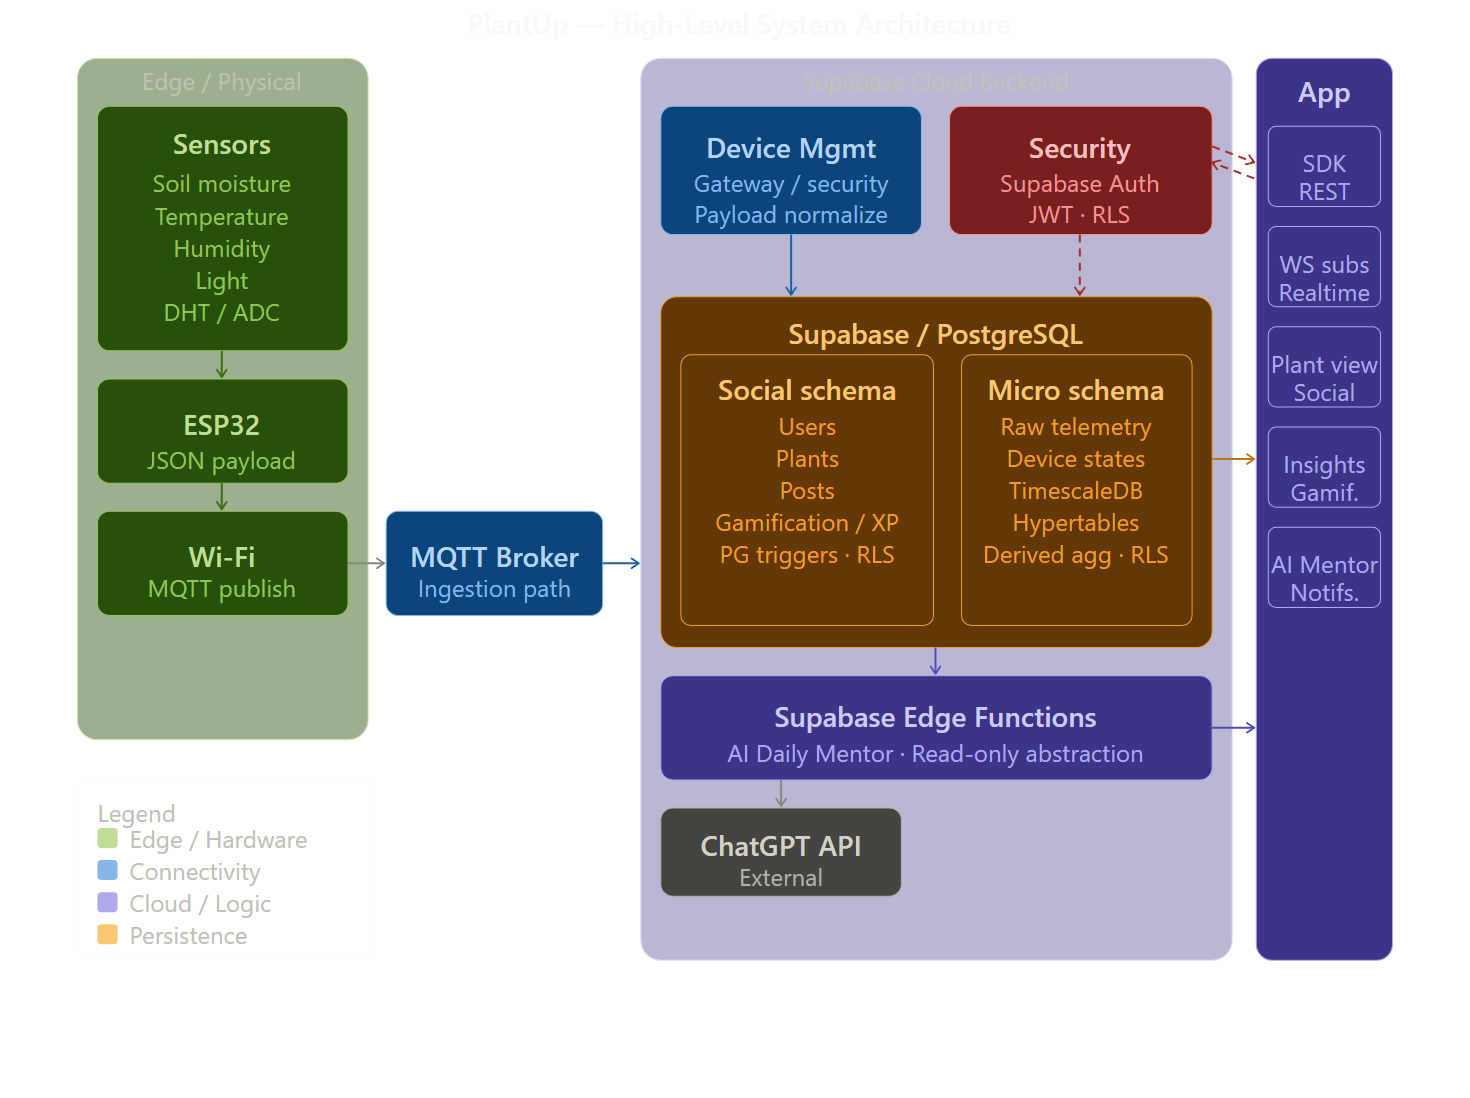
\includegraphics[width=0.85\textwidth,height=0.45\textheight,keepaspectratio]{Abudi/figures/plantup_fig1_master_v2.png}
    \caption{Master Architecture illustrating the chronological data pipeline. Source: Own work.}
    \label{fig:plantup_fig1_master}
\end{figure}

The architecture is designed strictly around the flow of telemetry: physical edge devices measure environmental data, transmit it to a scalable cloud backend, and the structured data is immediately made available to a React Native mobile application. 

\begin{wrapfigure}{R}{0.35\textwidth}
    \vspace{-15pt}
    \centering
    \scalebox{1.1}{\IoTNavigator{1}{0}{2}}
    \caption{Physical (Layer 1) and Connectivity (Layer 2) tiers of the Plant Up! telemetry pipeline. Source: Own work.}
    \vspace{-10pt}
\end{wrapfigure}
At the start of the pipeline is the physical layer, utilizing an ESP32 microcontroller deployed within the plant's environment. Acting as a pure ``Thin Edge'' component, the ESP32 performs no local computational analysis. Instead, it interfaces with analog and digital sensors to measure environmental metrics, including soil moisture, temperature, humidity, and light intensity, structures them into standardized JSON payloads, and transmits them for remote processing. 

The initial connectivity relies on Wi-Fi and MQTT for device-to-cloud communication. Direct device-to-smartphone technologies, such as Bluetooth Low Energy (BLE), were deliberately excluded because they limit real-time remote accessibility and can increase user friction. This Wi-Fi-to-Cloud pipeline supports a seamless global onboarding and monitoring experience. A quantitative performance benchmark of the MQTT protocol for this pipeline is evaluated in Chapter 4

In relation to the Cisco 7-Layer IoT reference model, the architecture cleanly partitions its concerns: the ESP32 acts strictly as Layer 1 (Physical Devices) communicating over Layer 2 (Connectivity), bypassing traditional Layer 3 Edge Computing entirely. The Supabase cloud environment manages Layer 4 (Data Accumulation) and Layer 5 (Data Abstraction), while the business logic and user collaboration occur within the application and client systems (Layers 6 and 7).

\subsection{Device Management and Ingestion}

Following the data flow, the incoming telemetry structured by the ESP32 must be securely received and translated into the persistence layer. To manage this safely without exposing internal database structures, the system incorporates a Device Management Service.

\begin{figure}[htbp]
    \centering
    \scalebox{1.25}{\IoTNavigator{2}{0}{0}}
    \caption{Highlight of the Ingestion Gateway within the architecture. Source: Own work.}
    \label{fig:ingestion_gateway}
\end{figure}

By actively buffering and processing high-velocity MQTT payloads from the broker, the C\# Middleware translates raw hardware telemetry (visualized in Figure~\ref{fig:csharp_ingestion_logic}), including connectivity states, registration data, and sensor measurements, into standardized database inserts. This layer serves as a secure translation boundary, catching the continuous stream of messages from the ESP32 and packaging them for the database. This abstraction protects the frontend application from underlying protocol complexities and isolates any hardware-level network issues from impacting user-facing application layers.

\begin{figure}[htbp]
    \centering
    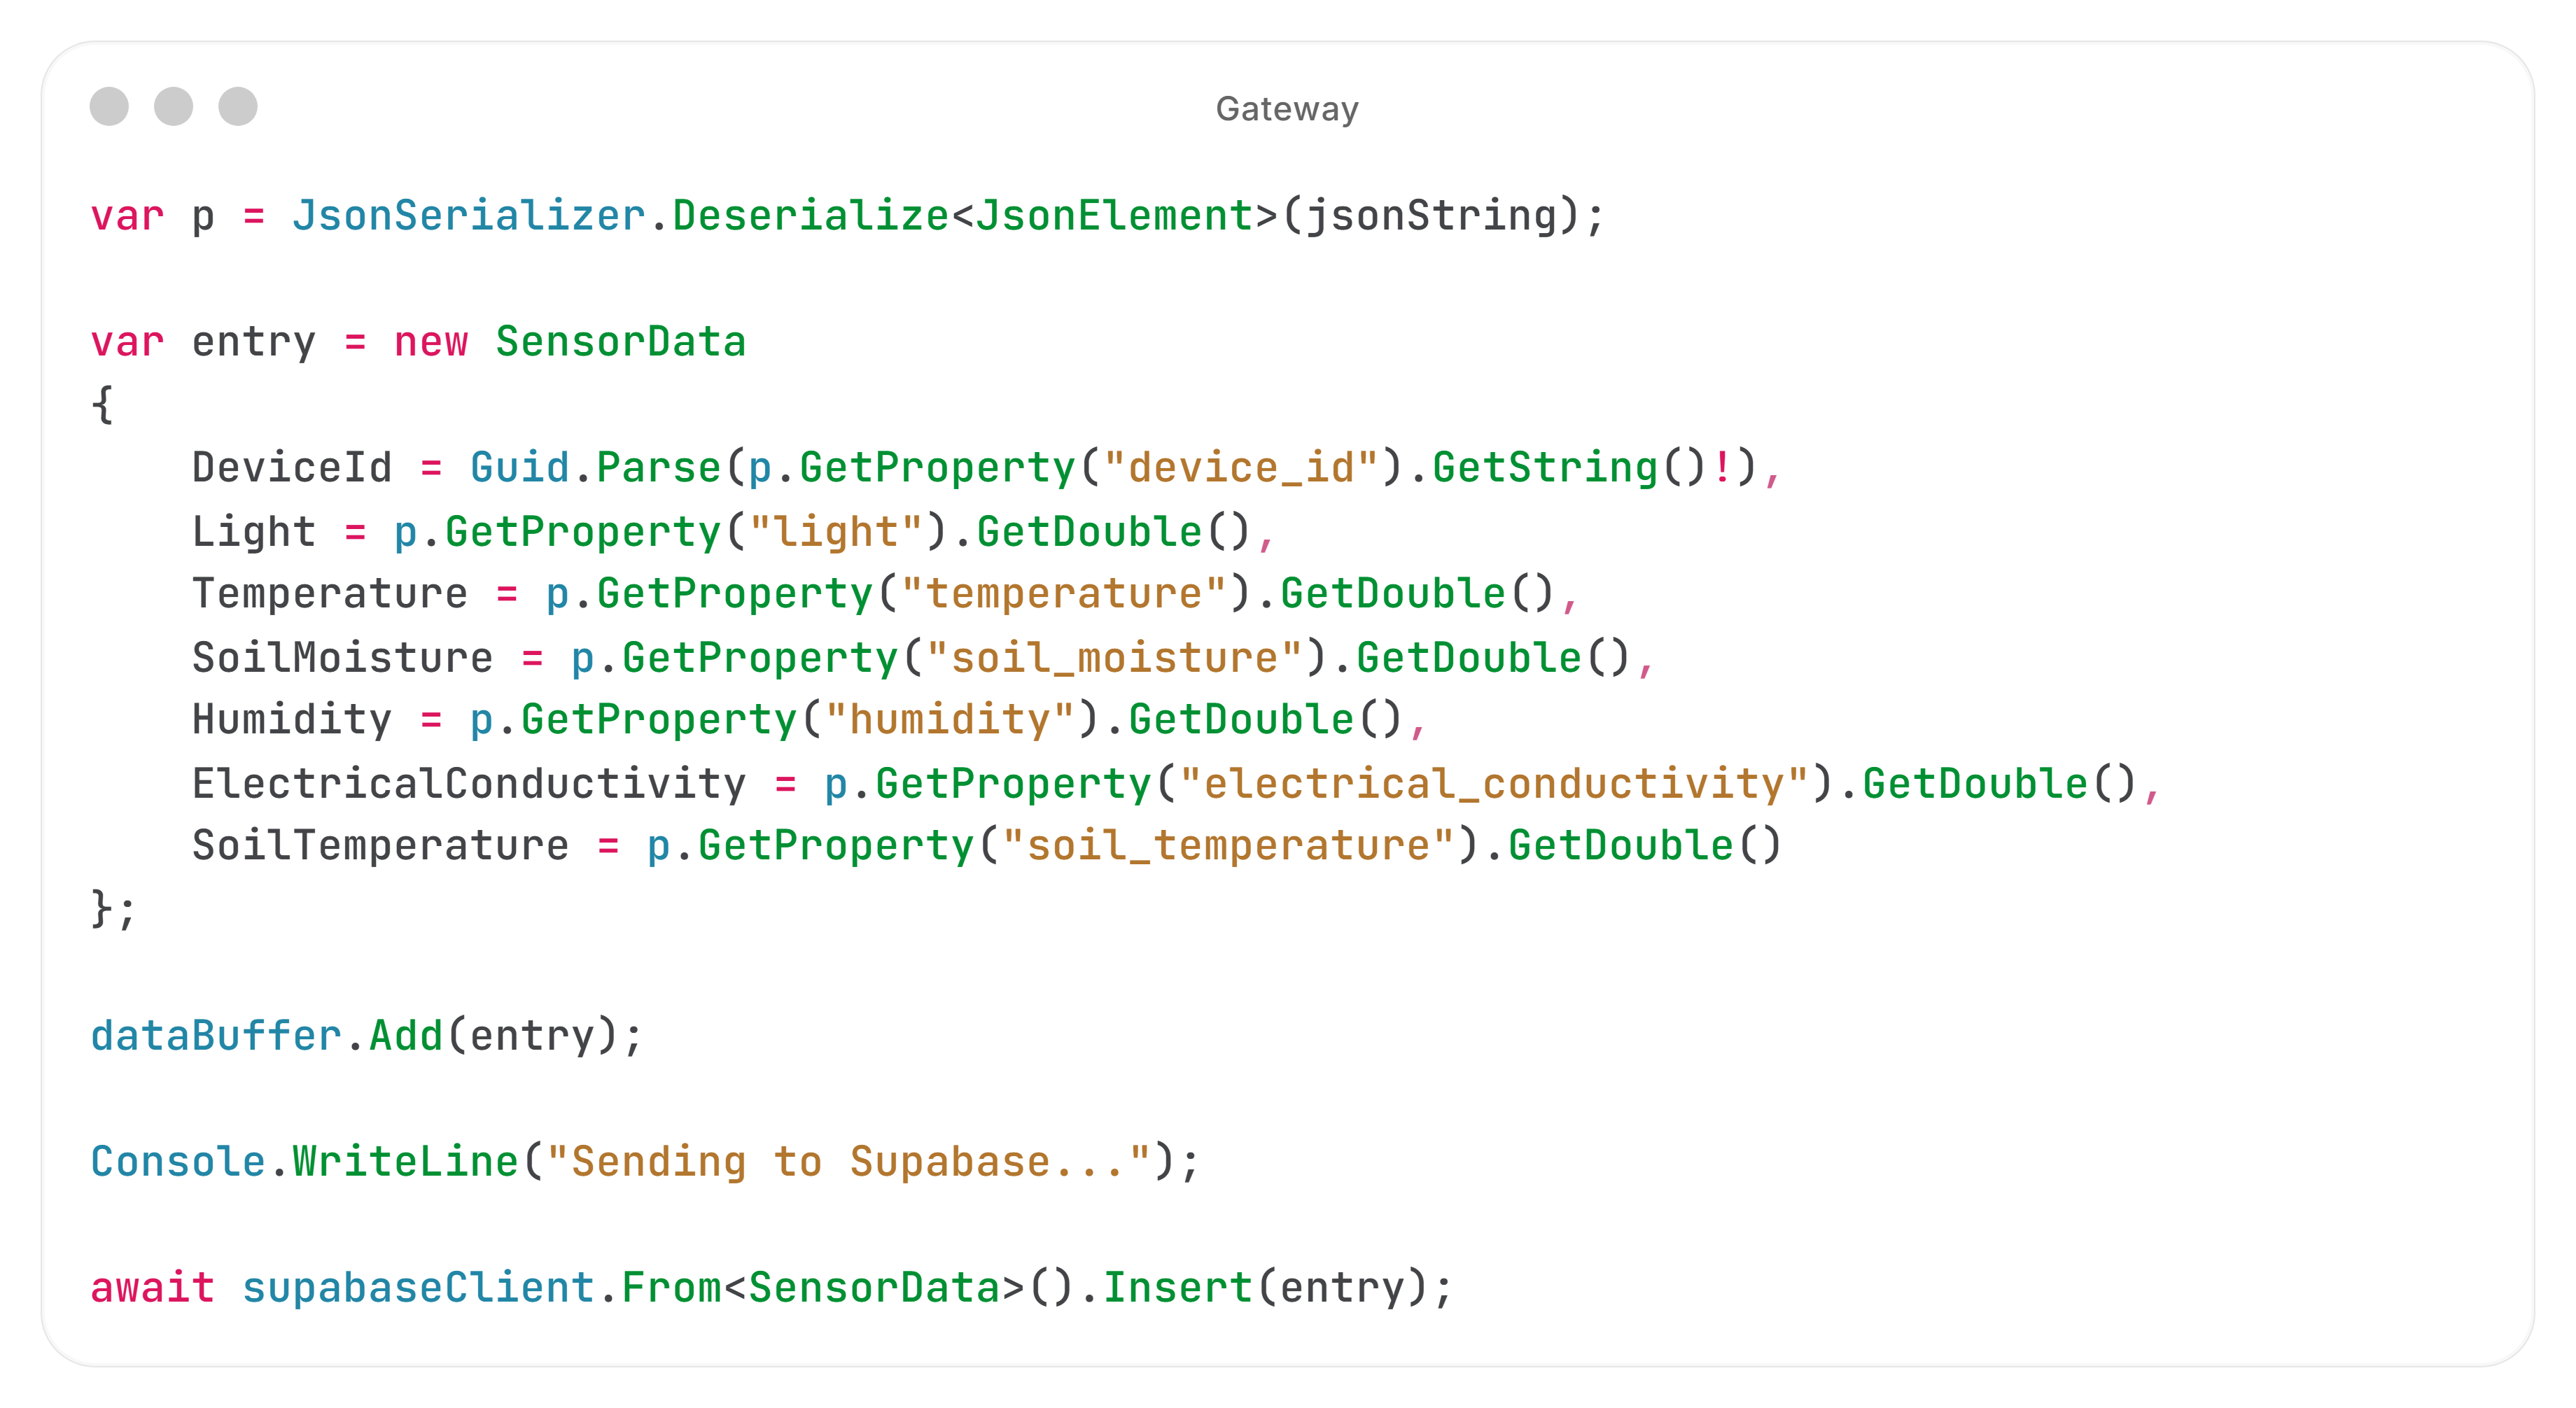
\includegraphics[width=0.85\textwidth]{Abudi/figures/Gateway.png}
    \caption{C\# Ingestion Middleware: Concurrent queue and batching logic responsible for buffering high-velocity sensor data. Source: Own work.}
    \label{fig:csharp_ingestion_logic}
\end{figure}



\subsection{The Data Persistence Layer (Supabase)}

Once telemetry passes the ingestion boundary, raw, unstructured data streams must be converted into durable, queryable formats. To manage relational application states, continuous telemetry, and user-generated social objects simultaneously, Plant Up! utilizes a consolidated PostgreSQL environment provided exclusively through Supabase.

\begin{figure}[htbp]
    \centering
    \scalebox{1.25}{\IoTNavigator{5}{0}{0}}
    \caption{Highlight of the Cloud Data Persistence layer within the architecture. Source: Own work.}
    \label{fig:persistence_layer}
\end{figure}
To prevent disparate data domains from conflating, the database fundamentally partitions data into two distinct logical schemas. The \textit{Social} schema securely manages user accounts, gamification progression, and interaction metrics. The \textit{Micro} schema serves purely as a telemetry repository, strictly dedicated to environmental sensor logs and historical analysis. 

While schema isolation effectively organizes relational data, processing the sheer volume of continuous telemetry generated by numerous physical devices requires structural optimization. To achieve this, telemetry measurements are ingested into TimescaleDB hypertables. TimescaleDB transparently partitions raw data into temporal chunks (e.g., grouping the last 24 hours of data), drastically reducing the indexing burden on the server. By querying only the active temporal chunks, the backend maintains consistently high retrieval speeds for the mobile application, even as the global database volume scales.



\subsection{Application Layer Services and Client Integration}

With the persistence layer firmly established, the final stage in the architecture focuses on business logic execution and mobile client connectivity. Instead of deploying a standalone intermediate web server, the application layer utilizes serverless functions and native database mechanisms structurally integrated within the Supabase ecosystem.

\begin{figure}[htbp]
    \centering
    \scalebox{1.25}{\IoTNavigator{7}{0}{0}}
    \caption{Highlight of the Application and Collaboration layer within the architecture. Source: Own work.}
    \label{fig:application_layer}
\end{figure}
To optimize state changes, the gamification engine utilizes native PostgreSQL triggers. Rather than requiring an active middle-tier polling service to constantly monitor user points, these triggers automate state progressions directly within the persistence layer upon predefined events, guaranteeing immediate data reconciliation and reducing architectural overhead. Similarly, AI-driven insights utilize serverless Supabase Edge Functions. When an insight is requested or triggered on a schedule, an ephemeral environment wakes up, queries recent telemetry from TimescaleDB, and interacts with external artificial intelligence APIs without clogging the primary database threads.

To seamlessly deliver this analyzed data to the user, the React Native mobile application adopts a direct-to-database architectural paradigm. Using the official Supabase SDK, the app establishes secure REST and WebSocket connections directly to the respective PostgreSQL schemas. Comprehensive security is maintained through Supabase Authentication combined with JSON Web Tokens (JWT). Most crucially, access control is enforced natively via Row-Level Security (RLS) policies within PostgreSQL, ensuring that the client application can only ever query or modify data explicitly tied to the authenticated user's ID \cite{broadwaySupabase, supabaseReactNative, tigerdataRelational}.

To empirically validate the efficiency of this architecture, particularly the latency trade-offs and database performance, the following section outlines the experimental methodology utilized for stress-testing the ``Thin Edge'' implementation.
